
\appendix
\renewcommand{\thesection}{SI \arabic{section}}
\setcounter{table}{0}\renewcommand\thetable{\thesection.\arabic{table}}
\setcounter{figure}{0}\renewcommand\thefigure{\thesection.\arabic{figure}}
\counterwithin{figure}{section}


\begin{center}
\Large \textbf{Supporting Information}
\end{center}
\singlespacing
\vspace{-.4in}

\section{Balance Tests}\label{si:baltests}

\begin{center}
	\begin{figure}[H]
		\centering
		\caption{MTurk 1---IDA and CUD}
		\includegraphics[width=\textwidth]{../figs/study1-baltest-RW-ips.pdf}
		\label{fig:baltest-RW-ips}
		\caption*{\footnotesize 
			Figure shows the balance tests of respondent characteristics for the Amazon Mechanical Turk Study 1 sample.
			The tests compare respondents assigned to the IDA condition vs. respondents assigned to the CUD condition.
			See \cref{tab:conditions} in \nameref{sec:inflationary_measures}.
			Rows are self-reported characteristics.
		      The second column reports the estimates from regressing the characteristics on the CUD dummy, with IDA as the baseline.
		      The third column reports the p-values.
			Horizontal bars are 95\% confidence intervals constructed from robust standard errors.
		}
	\end{figure}
\end{center}

% MTurk 1 balance test: IDA vs FSR (IPS vs FSR)
\begin{center}
	\begin{figure}
		\centering
		\caption{MTurk 1---IDA and FSR}
		\includegraphics[width=\textwidth]{../figs/study1-baltest-FSR-ips.pdf}
		\label{fig:baltest-FSR-ips}
		\caption*{\footnotesize 
			Figure shows the balance tests of respondent characteristics for the Amazon Mechanical Turk Study 1 sample.
			The tests compare respondents assigned to the IDA condition vs. respondents assigned to the FSR condition.
			See \cref{tab:conditions} in \nameref{sec:inflationary_measures}.
			Rows are self-reported characteristics.
			The second column reports the estimates from regressing the characteristics on the FSR dummy, with IDA as the baseline.
			The third column reports the p-values.
			Horizontal bars are 95\% confidence intervals constructed from robust standard errors.
		}
	\end{figure}
\end{center}

\begin{center}
	\begin{figure}
		\centering
		\caption{MTurk 1---IDA and IMC}
		\includegraphics[width=\textwidth]{../figs/study1-baltest-14k-ips.pdf}
		\label{fig:baltest-14k-ips}
		\caption*{\footnotesize 
			Figure shows the balance tests of respondent characteristics for the Amazon Mechanical Turk Study 1 sample.
			The tests compare respondents assigned to the IDA condition vs. respondents assigned to the IMC condition.
			See \cref{tab:conditions} in \nameref{sec:inflationary_measures}.
			Rows are self-reported characteristics.
			The second column reports the estimates from regressing the characteristics on the IMC dummy, with IDA as the baseline.
			The third column reports the p-values.
			Horizontal bars are 95\% confidence intervals constructed from robust standard errors.
		}
	\end{figure}
\end{center}

\begin{center}
	\begin{figure}
		\centering
		\caption{MTurk 1---IDA and CCD}
		\includegraphics[width=\textwidth]{../figs/study1-baltest-24k-ips.pdf}
		\label{fig:baltest-24k-ips}
		\caption*{\footnotesize 
			Figure shows the balance tests of respondent characteristics for the Amazon Mechanical Turk Study 1 sample.
			The tests compare respondents assigned to the IDA condition vs. respondents assigned to the CCD condition.
			See \cref{tab:conditions} in \nameref{sec:inflationary_measures}.
			Rows are self-reported characteristics.
			The second column reports the estimates from regressing the characteristics on the CCD dummy, with IDA as the baseline.
			The third column reports the p-values.
			Horizontal bars are 95\% confidence intervals constructed from robust standard errors.
		}
	\end{figure}
\end{center}

\section{Partisan Knowledge Gaps with Partisan Cues: YouGov}

\begin{figure}[ht]
	\caption{Partisan Knowledge Gaps with Partisan Cues: YouGov}
	\centering
	\begin{subfigure}{.495\textwidth}\centering
		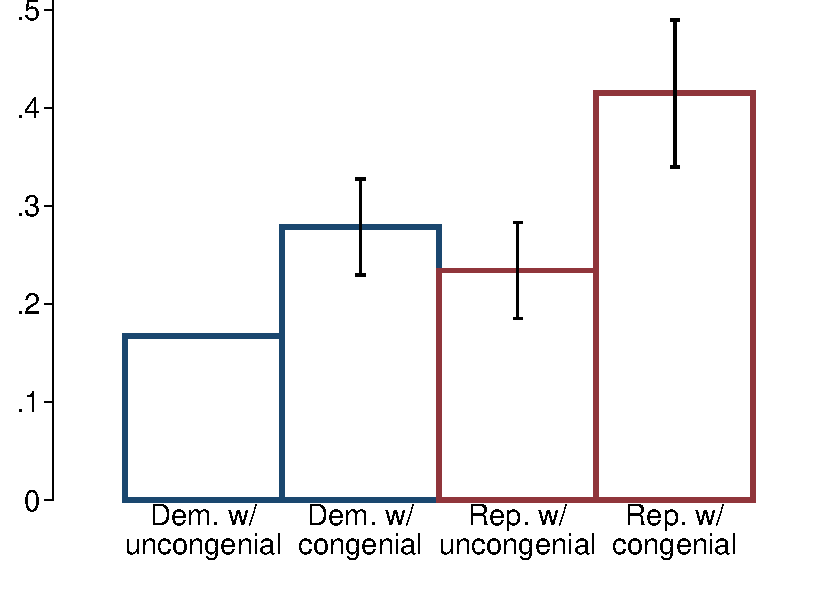
\includegraphics[width=\textwidth]{../figs/yougov-unemp-congenialcue-partisan.pdf}
		\caption{Unemployment}
	\end{subfigure}
	\hfil
	\begin{subfigure}{.495\textwidth}\centering
		\includegraphics[width=\textwidth]{../figs/yougov-deficit-congenialcue-partisan.pdf}
		\caption{Budget deficit}
	\end{subfigure}
	\caption*{\footnotesize Figure shows the effect of congenial cues for the YouGov survey by partisanship. Bars indicate the predicted percent of responses saying that unemployment has gone up (correct response) as retrieved from the estimates in \cref{tab:partisangaps-yougov} (columns (2) and (5)).  The estimates are obtained by estimating:\\

	$\qquad\text{correct response}_{i} = \alpha + \beta (congenial \; cue)_i + \gamma (Rep)_i + \delta (congenial\; cue \times Rep)_i + \varepsilon_{i}$.\\

	Capped vertical bars indicate 95\% confidence intervals.
	}
	\label{fig:yougov-reg-by-partisanship}
\end{figure}

\clearpage
\section{Confidence Scoring for Mturk 1}\label{si:mturk1-ccd}

\begin{table}[th] \centering \small \setlength\tabcolsep{0 pt} \setlength{\defaultaddspace}{0pt}
	\def\sym#1{\ifmmode^{#1}\else\(^{#1}\)\fi}
	\caption{Confidence Scoring vs. Other Survey Conditions (MTurk 1)}
	\label{tab:confidence-scoring-study1}
	\begin{adjustbox}{max width=\textwidth}
		\begin{tabular}{l*{10}{D{.}{.}{-1}}}
			\toprule
			&\multicolumn{1}{c}{Obama}
			&\multicolumn{1}{c}{Obama}
			&\multicolumn{1}{c}{ACA}
			&\multicolumn{1}{c}{ACA death}
			&\multicolumn{1}{c}{GW causes}
			&\multicolumn{1}{c}{GW scientists}
			&\multicolumn{1}{c}{Voter}
			&\multicolumn{1}{c}{MMR}
			&\multicolumn{1}{c}{Budget}
			&\multicolumn{1}{c}{}
			\\
			&\multicolumn{1}{c}{birthplace}
			&\multicolumn{1}{c}{religion}
			&\multicolumn{1}{c}{illegal}
			&\multicolumn{1}{c}{panels}
			&\multicolumn{1}{c}{GW causes}
			&\multicolumn{1}{c}{agree}
			&\multicolumn{1}{c}{fraud}
			&\multicolumn{1}{c}{vaccine}
			&\multicolumn{1}{c}{deficit}
			&\multicolumn{1}{c}{All}
			\\			
			\cmidrule(l){2-10}
			\input ../tabs/confidence-scoring-study1-fragment.tex
			\bottomrule
		\end{tabular}
	\end{adjustbox}
	\caption*{\scriptsize 
		All models are linear probability models where the dependent variable indicates whether the response to a survey item is correct.
		Under the Confidence Scoring condition, we only consider responses as correct when they are chosen with complete confidence (10 on a 0--10 scale).
		The baseline conditions are the IDA, CUD, FSR, and IMC conditions pooled together (see \cref{tab:conditions} for the descriptions).
		Columns (1)--(9) are for each of the survey questions.
		The model in column (10) pools all nine survey questions.
		See \cref{table:study4_results} for a similar result using MTurk 2.
		See \crefrange{tab:confidence-scoring-study1-ccd-ida-ips}{tab:confidence-scoring-study1-ccd-14k-imc} for the results comparing the Confidence Scoring condition to each of the four other individual survey conditions.
		See \cref{fig:confidence-scoring-study1} for the visualization of how Confidence Scoring mediates the effect that congenial responses have.
		Standard errors are clustered at the respondent level. 
		Significance levels: + 0.1 * 0.05 ** 0.01 *** 0.001.}
\end{table}

\begin{table}[t] \centering \small \setlength\tabcolsep{0 pt} \setlength{\defaultaddspace}{0pt}
	\def\sym#1{\ifmmode^{#1}\else\(^{#1}\)\fi}
	\caption{Confidence Scoring vs. IDA (MTurk 1)}
	\label{tab:confidence-scoring-study1-ccd-ida-ips}
	\begin{adjustbox}{max width=\textwidth}
		\begin{tabular}{l*{10}{D{.}{.}{-1}}}
			\toprule
			&\multicolumn{1}{c}{Obama}
			&\multicolumn{1}{c}{Obama}
			&\multicolumn{1}{c}{ACA}
			&\multicolumn{1}{c}{ACA death}
			&\multicolumn{1}{c}{GW causes}
			&\multicolumn{1}{c}{GW scientists}
			&\multicolumn{1}{c}{Voter}
			&\multicolumn{1}{c}{MMR}
			&\multicolumn{1}{c}{Budget}
			&\multicolumn{1}{c}{}
			\\
			&\multicolumn{1}{c}{birthplace}
			&\multicolumn{1}{c}{religion}
			&\multicolumn{1}{c}{illegal}
			&\multicolumn{1}{c}{panels}
			&\multicolumn{1}{c}{GW causes}
			&\multicolumn{1}{c}{agree}
			&\multicolumn{1}{c}{fraud}
			&\multicolumn{1}{c}{vaccine}
			&\multicolumn{1}{c}{deficit}
			&\multicolumn{1}{c}{All}
			\\			
			\cmidrule(l){2-10}
			\input ../tabs/confidence-scoring-study1-ccd-ida-ips-fragment.tex
			\bottomrule
		\end{tabular}
	\end{adjustbox}
	\caption*{\scriptsize 
		All models are linear probability models where the dependent variable indicates whether the response to a survey item is correct.
		Under the Confidence Scoring condition, we only consider responses as correct when they are chosen with complete confidence (10 on a 0--10 scale).
		The baseline condition is the IDA condition (see \cref{tab:conditions} for the descriptions).
		Columns (1)--(9) are for each of the survey questions.
		The model in column (10) pools all nine survey questions.
		See \cref{table:study4_results} for a similar result using MTurk 2.
		See \cref{tab:confidence-scoring-study1} for the results comparing the Confidence Scoring condition with all the four other conditions (IDA, CUD, FSR, IMC) pooled together.
		See \cref{fig:confidence-scoring-study1-ccd-ida-ips} for the visualization of how Confidence scoring mediates the effect that congenial responses have.
		See \cref{fig:confidence-scoring-study1-ccd-ida-ips} for the visualization of how Confidence scoring mediates the effect that congenial responses have.
		Standard errors are clustered at the respondent level. 
		Significance levels: + 0.1 * 0.05 ** 0.01 *** 0.001.}
\end{table}

\begin{table}[t] \centering \small \setlength\tabcolsep{0 pt} \setlength{\defaultaddspace}{0pt}
	\def\sym#1{\ifmmode^{#1}\else\(^{#1}\)\fi}
	\caption{Confidence Scoring vs. CUD (MTurk 1)}
	\label{tab:confidence-scoring-study1-ccd-rw-cud}
	\begin{adjustbox}{max width=\textwidth}
		\begin{tabular}{l*{10}{D{.}{.}{-1}}}
			\toprule
			&\multicolumn{1}{c}{Obama}
			&\multicolumn{1}{c}{Obama}
			&\multicolumn{1}{c}{ACA}
			&\multicolumn{1}{c}{ACA death}
			&\multicolumn{1}{c}{GW causes}
			&\multicolumn{1}{c}{GW scientists}
			&\multicolumn{1}{c}{Voter}
			&\multicolumn{1}{c}{MMR}
			&\multicolumn{1}{c}{Budget}
			&\multicolumn{1}{c}{}
			\\
			&\multicolumn{1}{c}{birthplace}
			&\multicolumn{1}{c}{religion}
			&\multicolumn{1}{c}{illegal}
			&\multicolumn{1}{c}{panels}
			&\multicolumn{1}{c}{GW causes}
			&\multicolumn{1}{c}{agree}
			&\multicolumn{1}{c}{fraud}
			&\multicolumn{1}{c}{vaccine}
			&\multicolumn{1}{c}{deficit}
			&\multicolumn{1}{c}{All}
			\\			
			\cmidrule(l){2-10}
			\input ../tabs/confidence-scoring-study1-ccd-cud-rw-fragment.tex
			\bottomrule
		\end{tabular}
	\end{adjustbox}
	\caption*{\scriptsize 
		All models are linear probability models where the dependent variable indicates whether the response to a survey item is correct.
		Under the Confidence Scoring condition, we only consider responses as correct when they are chosen with complete confidence (10 on a 0--10 scale).
		The baseline condition is the CUD condition (see \cref{tab:conditions} for the descriptions).
		Columns (1)--(9) are for each of the survey questions.
		The model in column (10) pools all nine survey questions.
		See \cref{table:study4_results} for a similar result using MTurk 2.
		See \cref{tab:confidence-scoring-study1} for the results comparing the Confidence scoring condition with all the four other conditions (IDA, CUD, FSR, IMC) pooled together.
		See \cref{fig:confidence-scoring-study1-ccd-rw-cud} for the visualization of how Confidence scoring mediates the effect that congenial responses have.
		Standard errors are clustered at the respondent level. 
		Significance levels: + 0.1 * 0.05 ** 0.01 *** 0.001.}
\end{table}


\begin{table}[t] \centering \small \setlength\tabcolsep{0 pt} \setlength{\defaultaddspace}{0pt}
	\def\sym#1{\ifmmode^{#1}\else\(^{#1}\)\fi}
	\caption{Confidence Scoring vs. FSR (MTurk 1)}
	\label{tab:confidence-scoring-study1-ccd-fsr-fsr}
	\begin{adjustbox}{max width=\textwidth}
		\begin{tabular}{l*{10}{D{.}{.}{-1}}}
			\toprule
			&\multicolumn{1}{c}{Obama}
			&\multicolumn{1}{c}{Obama}
			&\multicolumn{1}{c}{ACA}
			&\multicolumn{1}{c}{ACA death}
			&\multicolumn{1}{c}{GW causes}
			&\multicolumn{1}{c}{GW scientists}
			&\multicolumn{1}{c}{Voter}
			&\multicolumn{1}{c}{MMR}
			&\multicolumn{1}{c}{Budget}
			&\multicolumn{1}{c}{}
			\\
			&\multicolumn{1}{c}{birthplace}
			&\multicolumn{1}{c}{religion}
			&\multicolumn{1}{c}{illegal}
			&\multicolumn{1}{c}{panels}
			&\multicolumn{1}{c}{GW causes}
			&\multicolumn{1}{c}{agree}
			&\multicolumn{1}{c}{fraud}
			&\multicolumn{1}{c}{vaccine}
			&\multicolumn{1}{c}{deficit}
			&\multicolumn{1}{c}{All}
			\\			
			\cmidrule(l){2-10}
			\input ../tabs/confidence-scoring-study1-ccd-fsr-fsr-fragment.tex
			\bottomrule
		\end{tabular}
	\end{adjustbox}
	\caption*{\scriptsize 
		All models are linear probability models where the dependent variable indicates whether the response to a survey item is correct.
		Under the Confidence Scoring condition, we only consider responses as correct when they are chosen with complete confidence (10 on a 0--10 scale).
		The baseline condition is the FSR condition (see \cref{tab:conditions} for the descriptions).
		Columns (1)--(9) are for each of the survey questions.
		The model in column (10) pools all nine survey questions.
		See \cref{table:study4_results} for a similar result using MTurk 2.
		See \cref{tab:confidence-scoring-study1} for the results comparing the Confidence Scoring condition with all the four other conditions (IDA, CUD, FSR, IMC) pooled together.
		See \cref{fig:confidence-scoring-study1-ccd-fsr-fsr} for the visualization of how Confidence Scoring mediates the effect that congenial responses have.
		Standard errors are clustered at the respondent level. 
		Significance levels: + 0.1 * 0.05 ** 0.01 *** 0.001.}
\end{table}


\begin{table}[t] \centering \small \setlength\tabcolsep{0 pt} \setlength{\defaultaddspace}{0pt}
	\def\sym#1{\ifmmode^{#1}\else\(^{#1}\)\fi}
	\caption{Confidence Scoring vs. IMC (MTurk 1)}
	\label{tab:confidence-scoring-study1-ccd-14k-imc}
	\begin{adjustbox}{max width=\textwidth}
		\begin{tabular}{l*{10}{D{.}{.}{-1}}}
			\toprule
			&\multicolumn{1}{c}{Obama}
			&\multicolumn{1}{c}{Obama}
			&\multicolumn{1}{c}{ACA}
			&\multicolumn{1}{c}{ACA death}
			&\multicolumn{1}{c}{GW causes}
			&\multicolumn{1}{c}{GW scientists}
			&\multicolumn{1}{c}{Voter}
			&\multicolumn{1}{c}{MMR}
			&\multicolumn{1}{c}{Budget}
			&\multicolumn{1}{c}{}
			\\
			&\multicolumn{1}{c}{birthplace}
			&\multicolumn{1}{c}{religion}
			&\multicolumn{1}{c}{illegal}
			&\multicolumn{1}{c}{panels}
			&\multicolumn{1}{c}{GW causes}
			&\multicolumn{1}{c}{agree}
			&\multicolumn{1}{c}{fraud}
			&\multicolumn{1}{c}{vaccine}
			&\multicolumn{1}{c}{deficit}
			&\multicolumn{1}{c}{All}
			\\			
			\cmidrule(l){2-10}
			\input ../tabs/confidence-scoring-study1-ccd-imc-14k-fragment.tex
			\bottomrule
		\end{tabular}
	\end{adjustbox}
	\caption*{\scriptsize 
		All models are linear probability models where the dependent variable indicates whether the response to a survey item is correct.
		Under the Confidence Scoring condition, we only consider responses as correct when they are chosen with complete confidence (10 on a 0--10 scale).
		The baseline condition is the IMC condition (see \cref{tab:conditions} for the descriptions).
		Columns (1)--(9) are for each of the survey questions.
		The model in column (10) pools all nine survey questions.
		See \cref{table:study4_results} for a similar result using MTurk 2.
		See \cref{tab:confidence-scoring-study1} for the results comparing the Confidence Scoring condition with all the four other conditions (IDA, CUD, FSR, IMC) pooled together.
		See \cref{fig:confidence-scoring-study1-ccd-imc-14k} for the visualization of how Confidence Scoring mediates the effect that congenial responses have.
		Standard errors are clustered at the respondent level. 
		Significance levels: + 0.1 * 0.05 ** 0.01 *** 0.001.}
\end{table}


\begin{figure}[t]
	\caption{Confidence Scoring vs. Other Survey Conditions (MTurk 1)}	
	\centering
	% First row a
	\begin{subfigure}{.325\textwidth}\centering
		\includegraphics[width=\textwidth]{../figs/confidence_score_birth_study1.pdf}
		\caption{Obama birthplace}
	\end{subfigure}
	\hfill
	% First row b
	\begin{subfigure}{.325\textwidth}\centering
		\includegraphics[width=\textwidth]{../figs/confidence_score_religion_study1.pdf}
		\caption{Obama religion}
	\end{subfigure}	
	\hfill
	% First row c
	\begin{subfigure}{.325\textwidth}\centering
		\includegraphics[width=\textwidth]{../figs/confidence_score_illegal_study1.pdf}
		\caption{ACA illegal}
	\end{subfigure}	
	% Second row a
	\begin{subfigure}{.325\textwidth}\centering
		\includegraphics[width=\textwidth]{../figs/confidence_score_death_study1.pdf}
		\caption{ACA death panels}
	\end{subfigure}
	\hfill
	% Second row b
	\begin{subfigure}{.325\textwidth}\centering
		\includegraphics[width=\textwidth]{../figs/confidence_score_increase_study1.pdf}
		\caption{GW causes}
	\end{subfigure}	
	\hfill
	% Second row c
	\begin{subfigure}{.325\textwidth}\centering
		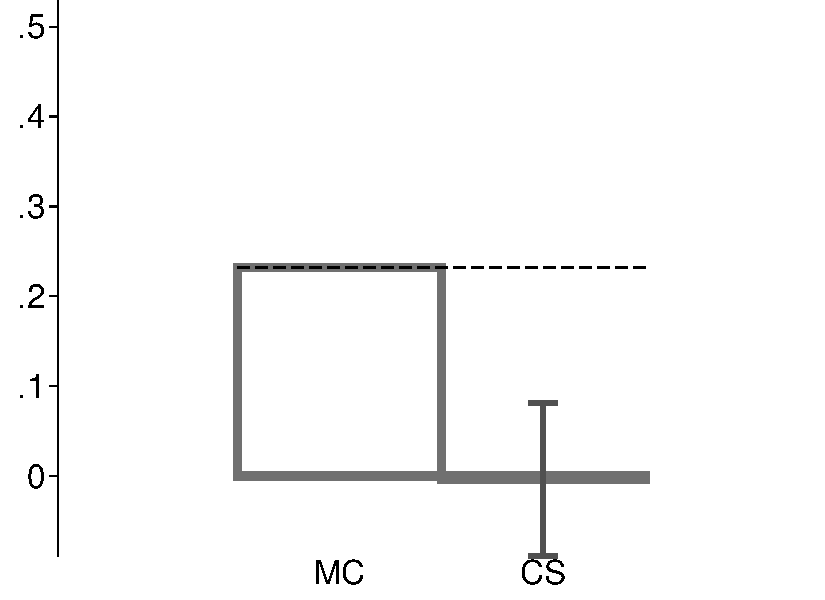
\includegraphics[width=\textwidth]{../figs/confidence_score_science_study1.pdf}
		\caption{GW scientists agree}
	\end{subfigure}	
	% Third row a
	\begin{subfigure}{.325\textwidth}\centering
		\includegraphics[width=\textwidth]{../figs/confidence_score_fraud_study1.pdf}
		\caption{Voter fraud}
	\end{subfigure}
	\hfill
	% Third row b
	\begin{subfigure}{.325\textwidth}\centering
		\includegraphics[width=\textwidth]{../figs/confidence_score_mmr_study1.pdf}
		\caption{MMR vaccine}
	\end{subfigure}	
	\hfill
	% Third row c
	\begin{subfigure}{.325\textwidth}\centering
		\includegraphics[width=\textwidth]{../figs/confidence_score_deficit_study1.pdf}
		\caption{Budget deficit}
	\end{subfigure}	
	\caption*{\footnotesize 
		Bars indicate the predicted percent of correct responses when the correct response is congenial to the party, depending on whether the survey condition is based on Confidence Scoring (CS) or from Multiple Choice conditions (IDA, CUD, FSR, IMC; see \cref{tab:conditions} for the descriptions).
		Reconstructed from the estimates from \cref{tab:confidence-scoring-study1}.
		Capped vertical bars indicate 95\% confidence intervals.
	}
	\label{fig:confidence-scoring-study1}
\end{figure}


\begin{figure}[t]
	\caption{Confidence Scoring vs. IDA (MTurk 1)}	
	\centering
	% First row a
	\begin{subfigure}{.325\textwidth}\centering
		\includegraphics[width=\textwidth]{../figs/confidence_score_ccd_ida_ips_birth_study1.pdf}
		\caption{Obama birthplace}
	\end{subfigure}
	\hfill
	% First row b
	\begin{subfigure}{.325\textwidth}\centering
		\includegraphics[width=\textwidth]{../figs/confidence_score_ccd_ida_ips_religion_study1.pdf}
		\caption{Obama religion}
	\end{subfigure}	
	\hfill
	% First row c
	\begin{subfigure}{.325\textwidth}\centering
		\includegraphics[width=\textwidth]{../figs/confidence_score_ccd_ida_ips_illegal_study1.pdf}
		\caption{ACA illegal}
	\end{subfigure}	
	% Second row a
	\begin{subfigure}{.325\textwidth}\centering
		\includegraphics[width=\textwidth]{../figs/confidence_score_ccd_ida_ips_death_study1.pdf}
		\caption{ACA death panels}
	\end{subfigure}
	\hfill
	% Second row b
	\begin{subfigure}{.325\textwidth}\centering
		\includegraphics[width=\textwidth]{../figs/confidence_score_ccd_ida_ips_increase_study1.pdf}
		\caption{GW causes}
	\end{subfigure}	
	\hfill
	% Second row c
	\begin{subfigure}{.325\textwidth}\centering
		\includegraphics[width=\textwidth]{../figs/confidence_score_ccd_ida_ips_science_study1.pdf}
		\caption{GW scientists agree}
	\end{subfigure}	
	% Third row a
	\begin{subfigure}{.325\textwidth}\centering
		\includegraphics[width=\textwidth]{../figs/confidence_score_ccd_ida_ips_fraud_study1.pdf}
		\caption{Voter fraud}
	\end{subfigure}
	\hfill
	% Third row b
	\begin{subfigure}{.325\textwidth}\centering
		\includegraphics[width=\textwidth]{../figs/confidence_score_ccd_ida_ips_mmr_study1.pdf}
		\caption{MMR vaccine}
	\end{subfigure}	
	\hfill
	% Third row c
	\begin{subfigure}{.325\textwidth}\centering
		\includegraphics[width=\textwidth]{../figs/confidence_score_ccd_ida_ips_deficit_study1.pdf}
		\caption{Budget deficit}
	\end{subfigure}	
	\caption*{\footnotesize 
		Bars indicate the predicted percent of correct responses when the correct response is congenial to the party, depending on whether the survey condition is based on Confidence Scoring (CS) or from multiple choice IDA condition (see \cref{tab:conditions} for the descriptions).
		Reconstructed from the estimates from \cref{tab:confidence-scoring-study1-ccd-ida-ips}.
		Capped vertical bars indicate 95\% confidence intervals.
	}
	\label{fig:confidence-scoring-study1-ccd-ida-ips}
\end{figure}


\begin{figure}[t]
	\caption{Confidence Scoring vs. CUD (MTurk 1)}	
	\centering
	% First row a
	\begin{subfigure}{.325\textwidth}\centering
		\includegraphics[width=\textwidth]{../figs/confidence_score_ccd_cud_rw_birth_study1.pdf}
		\caption{Obama birthplace}
	\end{subfigure}
	\hfill
	% First row b
	\begin{subfigure}{.325\textwidth}\centering
		\includegraphics[width=\textwidth]{../figs/confidence_score_ccd_cud_rw_religion_study1.pdf}
		\caption{Obama religion}
	\end{subfigure}	
	\hfill
	% First row c
	\begin{subfigure}{.325\textwidth}\centering
		\includegraphics[width=\textwidth]{../figs/confidence_score_ccd_cud_rw_illegal_study1.pdf}
		\caption{ACA illegal}
	\end{subfigure}	
	% Second row a
	\begin{subfigure}{.325\textwidth}\centering
		\includegraphics[width=\textwidth]{../figs/confidence_score_ccd_cud_rw_death_study1.pdf}
		\caption{ACA death panels}
	\end{subfigure}
	\hfill
	% Second row b
	\begin{subfigure}{.325\textwidth}\centering
		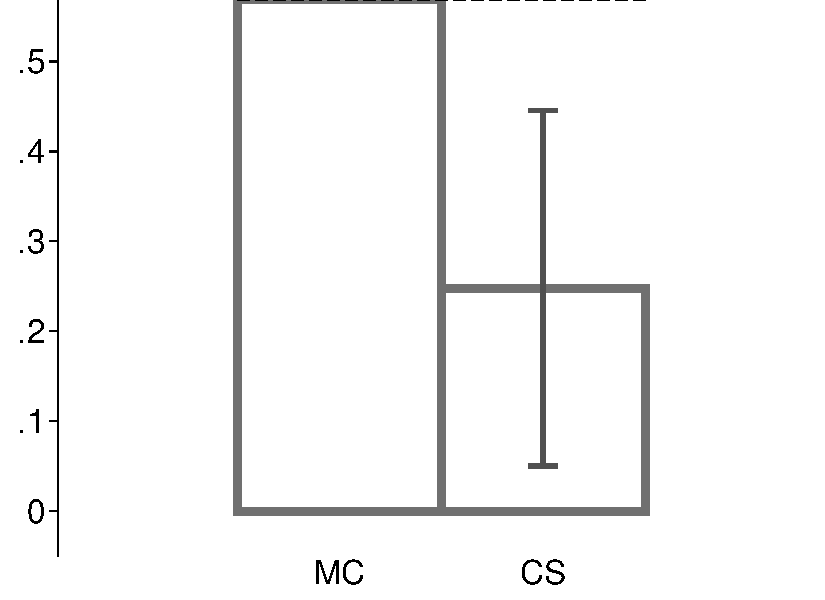
\includegraphics[width=\textwidth]{../figs/confidence_score_ccd_cud_rw_increase_study1.pdf}
		\caption{GW causes}
	\end{subfigure}	
	\hfill
	% Second row c
	\begin{subfigure}{.325\textwidth}\centering
		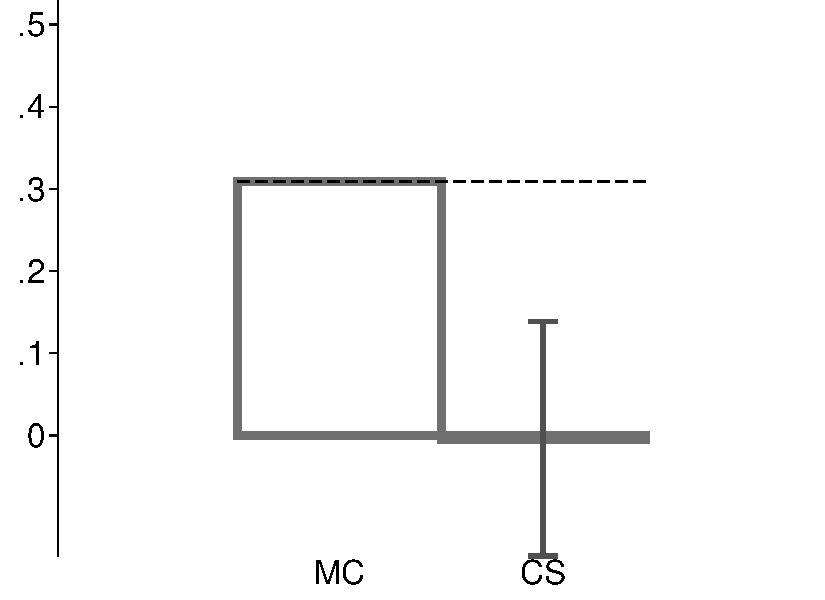
\includegraphics[width=\textwidth]{../figs/confidence_score_ccd_cud_rw_science_study1.pdf}
		\caption{GW scientists agree}
	\end{subfigure}	
	% Third row a
	\begin{subfigure}{.325\textwidth}\centering
		\includegraphics[width=\textwidth]{../figs/confidence_score_ccd_cud_rw_fraud_study1.pdf}
		\caption{Voter fraud}
	\end{subfigure}
	\hfill
	% Third row b
	\begin{subfigure}{.325\textwidth}\centering
		\includegraphics[width=\textwidth]{../figs/confidence_score_ccd_cud_rw_mmr_study1.pdf}
		\caption{MMR vaccine}
	\end{subfigure}	
	\hfill
	% Third row c
	\begin{subfigure}{.325\textwidth}\centering
		\includegraphics[width=\textwidth]{../figs/confidence_score_ccd_cud_rw_deficit_study1.pdf}
		\caption{Budget deficit}
	\end{subfigure}	
	\caption*{\footnotesize 
		Bars indicate the predicted percent of correct responses when the correct response is congenial to the party, depending on whether the survey condition is based on Confidence Scoring (CS) or from multiple choice CUD condition (see \cref{tab:conditions} for the descriptions).
		Reconstructed from the estimates from \cref{tab:confidence-scoring-study1-ccd-rw-cud}.
		Capped vertical bars indicate 95\% confidence intervals.
	}
	\label{fig:confidence-scoring-study1-ccd-rw-cud}
\end{figure}

\begin{figure}[t]
	\caption{Confidence Scoring vs. FSR (MTurk 1)}	
	\centering
	% First row a
	\begin{subfigure}{.325\textwidth}\centering
		\includegraphics[width=\textwidth]{../figs/confidence_score_ccd_fsr_fsr_birth_study1.pdf}
		\caption{Obama birthplace}
	\end{subfigure}
	\hfill
	% First row b
	\begin{subfigure}{.325\textwidth}\centering
		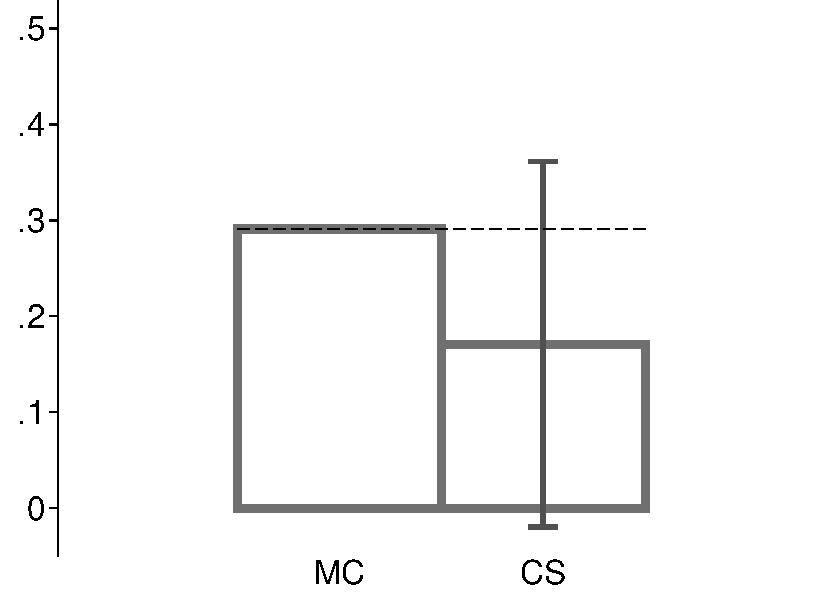
\includegraphics[width=\textwidth]{../figs/confidence_score_ccd_fsr_fsr_religion_study1.pdf}
		\caption{Obama religion}
	\end{subfigure}	
	\hfill
	% First row c
	\begin{subfigure}{.325\textwidth}\centering
		\includegraphics[width=\textwidth]{../figs/confidence_score_ccd_fsr_fsr_illegal_study1.pdf}
		\caption{ACA illegal}
	\end{subfigure}	
	% Second row a
	\begin{subfigure}{.325\textwidth}\centering
		\includegraphics[width=\textwidth]{../figs/confidence_score_ccd_fsr_fsr_death_study1.pdf}
		\caption{ACA death panels}
	\end{subfigure}
	\hfill
	% Second row b
	\begin{subfigure}{.325\textwidth}\centering
		\includegraphics[width=\textwidth]{../figs/confidence_score_ccd_fsr_fsr_increase_study1.pdf}
		\caption{GW causes}
	\end{subfigure}	
	\hfill
	% Second row c
	\begin{subfigure}{.325\textwidth}\centering
		\includegraphics[width=\textwidth]{../figs/confidence_score_ccd_fsr_fsr_science_study1.pdf}
		\caption{GW scientists agree}
	\end{subfigure}	
	% Third row a
	\begin{subfigure}{.325\textwidth}\centering
		\includegraphics[width=\textwidth]{../figs/confidence_score_ccd_fsr_fsr_fraud_study1.pdf}
		\caption{Voter fraud}
	\end{subfigure}
	\hfill
	% Third row b
	\begin{subfigure}{.325\textwidth}\centering
		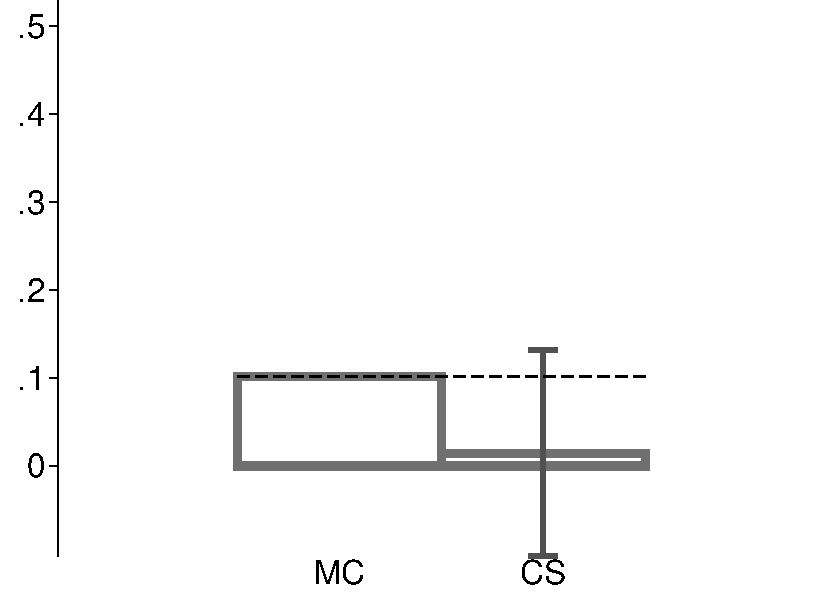
\includegraphics[width=\textwidth]{../figs/confidence_score_ccd_fsr_fsr_mmr_study1.pdf}
		\caption{MMR vaccine}
	\end{subfigure}	
	\hfill
	% Third row c
	\begin{subfigure}{.325\textwidth}\centering
		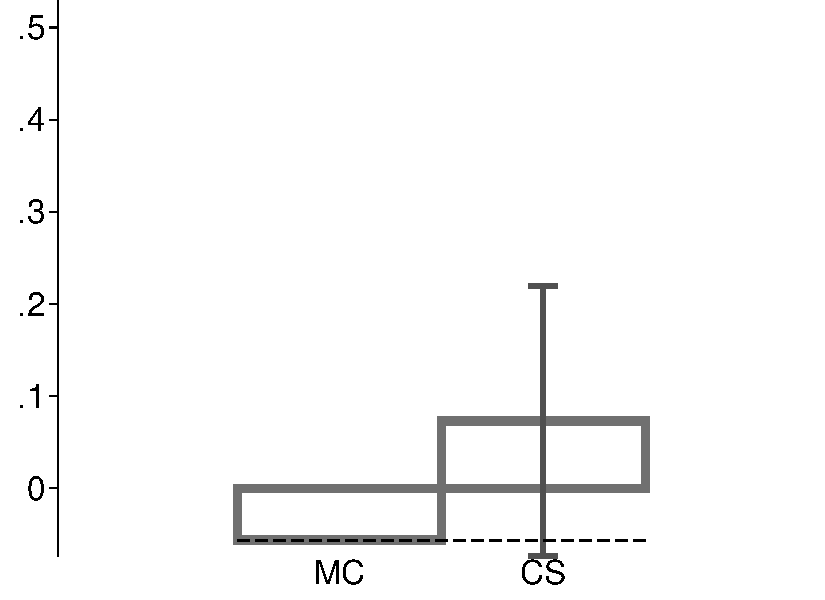
\includegraphics[width=\textwidth]{../figs/confidence_score_ccd_fsr_fsr_deficit_study1.pdf}
		\caption{Budget deficit}
	\end{subfigure}	
	\caption*{\footnotesize 
		Bars indicate the predicted percent of correct responses when the correct response is congenial to the party, depending on whether the survey condition is based on Confidence Scoring (CS) or from multiple choice CUD condition (see \cref{tab:conditions} for the descriptions).
		Reconstructed from the estimates from \cref{tab:confidence-scoring-study1-ccd-fsr-fsr}.
		Capped vertical bars indicate 95\% confidence intervals.
	}
	\label{fig:confidence-scoring-study1-ccd-fsr-fsr}
\end{figure}

\begin{figure}[t]
	\caption{Confidence Scoring vs. IMC (MTurk 1)}	
	\centering
	% First row a
	\begin{subfigure}{.325\textwidth}\centering
		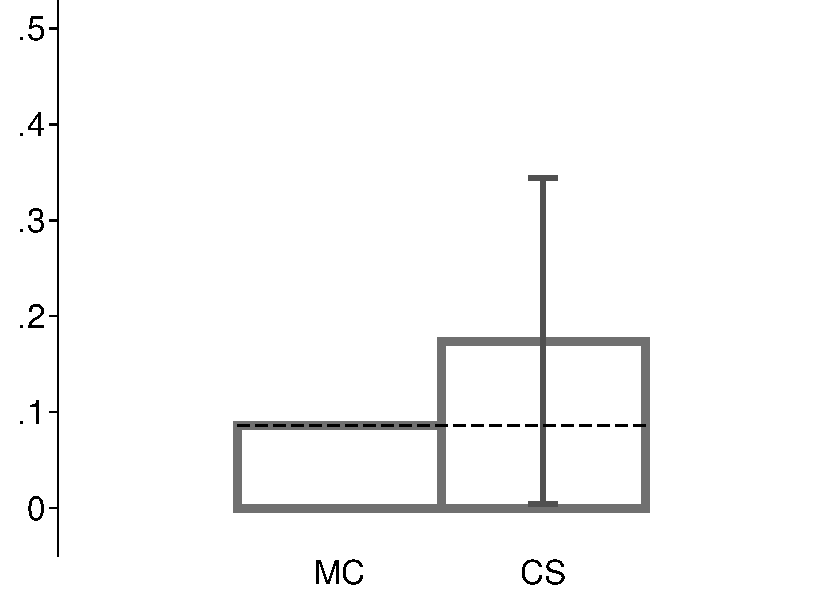
\includegraphics[width=\textwidth]{../figs/confidence_score_ccd_imc_14k_birth_study1.pdf}
		\caption{Obama birthplace}
	\end{subfigure}
	\hfill
	% First row b
	\begin{subfigure}{.325\textwidth}\centering
		\includegraphics[width=\textwidth]{../figs/confidence_score_ccd_imc_14k_religion_study1.pdf}
		\caption{Obama religion}
	\end{subfigure}	
	\hfill
	% First row c
	\begin{subfigure}{.325\textwidth}\centering
		\includegraphics[width=\textwidth]{../figs/confidence_score_ccd_imc_14k_illegal_study1.pdf}
		\caption{ACA illegal}
	\end{subfigure}	
	% Second row a
	\begin{subfigure}{.325\textwidth}\centering
		\includegraphics[width=\textwidth]{../figs/confidence_score_ccd_imc_14k_death_study1.pdf}
		\caption{ACA death panels}
	\end{subfigure}
	\hfill
	% Second row b
	\begin{subfigure}{.325\textwidth}\centering
		\includegraphics[width=\textwidth]{../figs/confidence_score_ccd_imc_14k_increase_study1.pdf}
		\caption{GW causes}
	\end{subfigure}	
	\hfill
	% Second row c
	\begin{subfigure}{.325\textwidth}\centering
		\includegraphics[width=\textwidth]{../figs/confidence_score_ccd_imc_14k_science_study1.pdf}
		\caption{GW scientists agree}
	\end{subfigure}	
	% Third row a
	\begin{subfigure}{.325\textwidth}\centering
		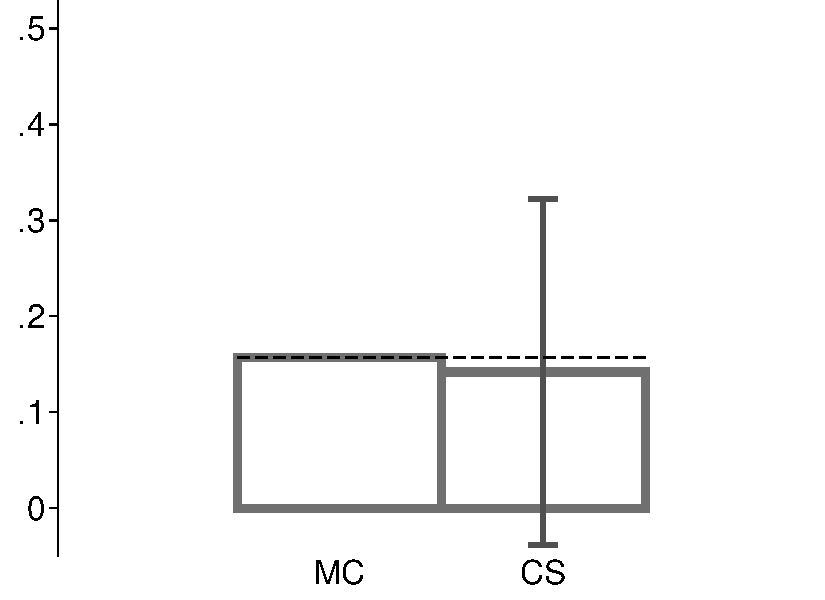
\includegraphics[width=\textwidth]{../figs/confidence_score_ccd_imc_14k_fraud_study1.pdf}
		\caption{Voter fraud}
	\end{subfigure}
	\hfill
	% Third row b
	\begin{subfigure}{.325\textwidth}\centering
		\includegraphics[width=\textwidth]{../figs/confidence_score_ccd_imc_14k_mmr_study1.pdf}
		\caption{MMR vaccine}
	\end{subfigure}	
	\hfill
	% Third row c
	\begin{subfigure}{.325\textwidth}\centering
		\includegraphics[width=\textwidth]{../figs/confidence_score_ccd_imc_14k_deficit_study1.pdf}
		\caption{Budget deficit}
	\end{subfigure}	
	\caption*{\footnotesize 
		Bars indicate the predicted percent of correct responses when the correct response is congenial to the party, depending on whether the survey condition is based on Confidence Scoring (CS) or from multiple choice CUD condition (see \cref{tab:conditions} for the descriptions).
		Reconstructed from the estimates from \cref{tab:confidence-scoring-study1-ccd-fsr-fsr}.
		Capped vertical bars indicate 95\% confidence intervals.
	}
	\label{fig:confidence-scoring-study1-ccd-imc-14k}
\end{figure}

\section{Partisan Gaps in Knowledge Across Question Designs}
\begin{center}
	\begin{figure}[ht]
		\centering
		\caption{Partisan Gaps in Knowledge Across Question Designs (Pooled multiple choices)}
		\includegraphics[width=.9\textwidth]{../figs/partisan-gap-by-item-arm-mc-24k.pdf}
		\label{fig:mturk_hk24_mc}
		\caption*{\footnotesize
		The figure shows the estimated partisan gaps in knowledge from the MTurk sample for Study 1 for the four multiple-choice survey conditions (pooling IDA, CUD, FSR, and IMC) and the confidence coding design (CCD). Corresponds to \cref{fig:mturk_hk24}.
            The CCD condition only considers selecting the right answer with complete confidence as evidence that the respondent knows the answer (see \cref{si:mturk2}).
            See \crefrange{tab:confidence-scoring-study1}{tab:confidence-scoring-study1-ccd-14k-imc} in \cref{si:mturk1-ccd} for the regression estimates of the multiple-choice conditions to the confidence coding condition.
		}
	\end{figure}
\end{center}

\clearpage
\section{Item Text for MTurk 1}\label{si:mturk1}
For exposition, we present the conditions using different terms in the main body (see \cref{tab:conditions}). The following shows how our terminologies for conditions map to the MTurk questionnaires.

\begin{itemize}
    \item{\textbf{IP} = \textbf{IDA}} 
    \item{\textbf{RW} = \textbf{CUD}} 
\end{itemize}

\noindent
\textbf{Preface for Different Conditions}

\textbf{RW, IP}\newline
Now here are some questions about what you may know about politics and public affairs.

\textbf{FSR, IMC, CCD}\newline
Now here are some questions about what you may know about politics and public affairs.
We are interested in measuring what people currently know and can recall on their own and are just as interested in what people don't know as in what they do know. So we'd like your agreement to just say ``don't know'' if you don't know the answer—without looking anything up or talking with anyone about it.

\textbf{Item Text}
\textbf{CCD}\newline
Now here are a series of statements. On a scale of 0 to 10, where 0 means definitely false, 10 means definitely true, and 5 is exactly in the middle, how definitely true or false is each statement?

\begin{itemize}
	\item Barack Obama was born in the US (T)
	\item  Barack Obama is a Muslim (F)
	\item  The Affordable Care Act gives illegal immigrants financial help to buy health insurance (F)
	\item  The Affordable Care Act does not create government panels to make decisions about end-of-life care (T)
	\item  Temperatures around the world are increasing because of human activity, like burning coal and gasoline (T)
	\item  Most climate scientists believe that global warming is not occurring (F)
	\item  In the 2016 presidential election, President Trump won the majority of the legally cast votes (F)
	\item  The vaccine for measles, mumps, and rubella (MMR) causes autism in children. (F)
	\item  Since 2012, the annual federal budget deficit has increased. (T)
\end{itemize}

\textbf{Rest of the Conditions, By Item}

\begin{itemize}
\item Obama's Birthplace

\textbf{RW and IP}\newline

According to the Constitution, American presidents must be ``natural-born citizens.''
Some people believe Barack Obama was not born in the United States but was born
in another country. Do you think Barack Obama was born in ...?
\begin{itemize}
	\item The US
	\item Another country
\end{itemize}

\textbf{FSR}\newline
Some people believe Barack Obama was not born in the United States but was born
in another country. Was he born in ...?
\begin{itemize}
	\item The US
	\item Another country
	\item DK (plus DK pref)
\end{itemize}

\textbf{IMC}\newline

Was Barack Obama born in ...?
\begin{itemize}
	\item the US
	\item Another country
	\item DK (plus DK pref)
\end{itemize}

\item Obama Religion\newline
\textbf{RW}\newline

Do you personally believe that Barack Obama is a ...?
\begin{itemize}
	\item Muslim
	\item Christian
\end{itemize}

\textbf{IP}\newline

Most people have a religion. Some people believe Barack Obama is a Muslim. Do you personally believe that Barack Obama is a \ldots?
\begin{itemize}
	\item Muslim
	\item Christian
\end{itemize}

\textbf{FSR}\newline

Some people believe Barack Obama is a Muslim. Is he a \ldots?
\begin{itemize}
	\item Muslim
	\item Christian
	\item DK (+ DK pref)
\end{itemize}

\textbf{IMC}\newline

Is Barack Obama a \ldots?
\begin{itemize}
	\item Muslim
	\item Christian
	\item DK (plus DK pref)
\end{itemize}

\item ACA Illegal\newline
\textbf{RW}\newline

To the best of your knowledge, would you say the Affordable Care Act \ldots?
\begin{itemize}
	\item Gives illegal immigrants financial help to buy health insurance
	\item Does not give illegal immigrants financial help to buy health insurance
\end{itemize}

\textbf{IP}\newline

As you may know, there is currently talk of changing the Affordable Care Act
(ACA), enacted in 2010. Some people believe that the ACA gives illegal immigrants
financial help to buy health insurance. To the best of your knowledge, would you say
the ACA\ldots?
\begin{itemize}
	\item Gives illegal immigrants financial help to buy health insurance
	\item Does not give illegal immigrants financial help to buy health insurance
\end{itemize}

\textbf{FSR}\newline

Some people believe that the Affordable Care Act gives illegal immigrants financial help
to buy health insurance. Does the Affordable Care Act \ldots?
\begin{itemize}
	\item Give illegal immigrants financial help to buy health insurance
	\item Not give illegal immigrants financial help to buy health insurance
	\item DK (+ DK pref)
\end{itemize}

\textbf{IMC}\newline
Does the Affordable Care Act \ldots?
\begin{itemize}
	\item Give illegal immigrants financial help to buy health insurance
	\item Not Give illegal immigrants financial help to buy health insurance
	\item Don't know (+ DK pref)
\end{itemize}

\item ACA—Death Panels\newline
\textbf{RW}\newline
To the best of your knowledge, would you say that the Affordable Care Act \ldots?
\begin{itemize}
	\item Creates government panels to make decisions about end-of-life care
	\item Does not create government panels to make decisions about end-of-life care
\end{itemize}

\textbf{IP}\newline

Some people believe that the Affordable Care Act establishes a government panel to
make decisions about end-of-life care. To the best of your knowledge, would you say
that the Affordable Care Act \ldots?
\begin{itemize}
	\item Creates government panels to make decisions about end-of-life care
	\item Does not create government panels to make decisions about end-of-life care
\end{itemize}

\textbf{FSR}\newline

Some people believe that the Affordable Care Act establishes a government panel to
make decisions about end-of-life care. Does the Affordable Care Act \ldots?
\begin{itemize}
	\item Creates government panels to make decisions about end-of-life care
	\item Does not create government panels to make decisions about end-of-life care
	\item DK (+ DK pref)
\end{itemize}

\textbf{IMC}\newline
Does the Affordable Care Act \ldots?
\begin{itemize}
	\item Creates government panels to make decisions about end-of-life care
	\item Does not create government panels to make decisions about end-of-life care
	\item DK (+ DK pref)
\end{itemize}

\item Global Warming—Happening + Causes\newline
\textbf{RW}\newline
Which of the following best fits your view about this? Are temperatures around the
world \ldots?
\begin{itemize}
	\item Increasing because of the natural variation over time, such as produced by the ice age
	\item Increasing because of human activity, like burning coal and gasoline
	\item Staying about the same as they have been
\end{itemize}

\textbf{IP}\newline
Recently, you may have noticed that global warming has been getting some attention
in the news. Some people believe that temperatures are increasing around the world
because of natural variation over time, such as that produced the ice age. Which of the
following best fits your view about this? Would you say that temperatures around the
world are\ldots?
\begin{itemize}
	\item Increasing because of the natural variation over time, such as produced by the ice age
	\item Increasing because of human activity, like burning coal and gasoline
	\item Staying about the same as they have been
\end{itemize}

\textbf{FSR}\newline

Some people believe that temperatures are increasing around the world because of
natural variation over time, such as produced the ice age. Are temperatures around
the world \ldots?
\begin{itemize}
	\item Increasing because of the natural variation over time, such as produced by the ice age
	\item Increasing because of human activity, like burning coal and gasoline
	\item Staying about the same as they have been
	\item DK (+ DK pref)
\end{itemize}

\textbf{IMC}\newline
Are temperatures around the world \ldots?
\begin{itemize}
	\item Increasing because of natural variation over time, such as produced by the ice age
	\item Increasing because human activity, like burning coal and gasoline
	\item Staying about the same as they have been
	\item DK (+ DK pref)
\end{itemize}

\item GW—Scientist Agreement\newline
\textbf{RW}\newline
Just your impression, which one of the following statements do you think is most
accurate?
\begin{itemize}
	\item Most climate scientists believe that global warming is occurring.
	\item Most climate scientists believe that global warming is not occurring.
	\item Climate scientists are about equally divided about whether global warming is occurring or not
\end{itemize}

\textbf{IP}\newline
As you may know, the term ``global warming'' refers to the claim that temperatures
have been increasing around the world. Some people believe that most climate
scientists believe that global warming is not occurring. Just your impression, which
one of the following statements do you think is most accurate?
\begin{itemize}
	\item Most climate scientists believe that global warming is occurring.
	\item Most climate scientists believe that global warming is not occurring.
	\item Climate scientists are about equally divided about whether global warming is occurring or not
\end{itemize}
\textbf{FSR}\newline
Some people believe that most climate scientists believe that global warming is not
occurring. Which one of the following statements is most accurate?
\begin{itemize}
	\item Most climate scientists believe that global warming is occurring.
	\item Most climate scientists believe that global warming is not occurring.
	\item Climate scientists are about equally divided about whether global warming is occurring or not
	\item DK (+ DK pref)
\end{itemize}

\textbf{IMC}\newline
Which one of the following statements is most accurate?
\begin{itemize}
	\item Most climate scientists believe that global warming is occurring.
	\item Most climate scientists believe that global warming is NOT occurring.
	\item Climate scientists are about equally divided about whether global warming is occurring or not
	\item DK (+ DK pref)
\end{itemize}

\item Voter Fraud\newline
\textbf{RW}\newline
As you may know, President Trump has said that several million people voted
illegally in the 2016 presidential election and that he won the majority of the legally
cast votes. Do you believe that President Trump \ldots?
\begin{itemize}
	\item Won the majority of the legally cast votes
	\item Did not win the majority of the legally cast votes
\end{itemize}

\textbf{IP}\newline
As you may know, not everyone living in the US has the legal right to vote. President
Trump has said that several million people voted illegally in the 2016 presidential
election and that he won the majority of the legally cast votes. Do think that
President Trump \ldots?
\begin{itemize}
	\item Won the majority of the legally cast votes
	\item Did not win the majority of the legally cast votes
\end{itemize}

\textbf{FSR}\newline
As you may know, President Trump has said that several million people voted
illegally in the 2016 presidential election and that he won the majority of the legally
cast votes. Did President Trump \ldots?
\begin{itemize}
	\item Won the majority of the legally cast votes
	\item Did not win the majority of the legally cast votes
	\item DK (+ DK pref)
\end{itemize}

\textbf{IMC}\newline
In the 2016 presidential election, did President Trump \ldots?
\begin{itemize}
	\item Won the majority of the legally cast votes
	\item Did not win the majority of the legally cast votes
	\item DK (+ DK pref)
\end{itemize}

\item Vaccines\newline
\textbf{RW}\newline
From what you have read or heard, do you personally think that the vaccine for
Measles, Mumps, and Rubella (MMR):
\begin{itemize}
	\item Causes autism in children
	\item Does not cause autism in children
\end{itemize}

\textbf{IP}\newline
As you may know, most children receive the vaccine for Measles, Mumps, and
Rubella (MMR). Some people believe that the MMR vaccine causes autism in
children. From what you have read or heard, do you personally think that the MMR
vaccine:
\begin{itemize}
	\item Causes autism in children
	\item Does not cause autism in children
\end{itemize}

\textbf{FSR}\newline
Some people believe that the vaccine for Measles, Mumps, and Rubella (MMR)
causes autism in children. Does the MMR vaccine \ldots?
\begin{itemize}
	\item Cause autism in children
	\item Not cause autism in children.
	\item DK (+ DK pref)
\end{itemize}

\textbf{IMC}\newline
Does the vaccine for Measles, Mumps, and Rubella (MMR) \ldots?
\begin{itemize}
	\item Cause autism in children
	\item Not cause autism in children.
	\item DK (+ DK pref)
\end{itemize}

\item Obama—Budget Deficit\newline
\textbf{RW}\newline
As you may know, the federal government runs a deficit when it spends more than it
takes in. Since 2012, would you say that the annual federal budget deficit has \ldots
\begin{itemize}
	\item Increased
	\item Stayed about the same
	\item Decreased
\end{itemize}

\textbf{IP}\newline
As you may know, the federal government runs a deficit when it spends more than it
takes in. Since 2012, with the Republicans having the majority in the U.S. House of
Representatives, would you say that the annual federal budget deficit has \ldots
\begin{itemize}
	\item Increased
	\item Stayed about the same
	\item Decreased
\end{itemize}

\textbf{FSR}\newline
Since 2012, with the Republicans having the majority in the U.S. House of
Representatives,
\begin{itemize}
	\item has the annual federal budget deficit \ldots.
	\item Increased
	\item Stayed about the same
	\item Decreased
	\item DK (+ DK pref)
\end{itemize}

\textbf{IMC}\newline

Since 2012, has the annual federal budget deficit \ldots
\begin{itemize}
	\item Increased
	\item Stayed about the same
	\item Decreased
	\item DK (+ DK pref)
\end{itemize}
\end{itemize}

\newpage

\clearpage
\section{Criterion Variables}\label{si:mturk1_criteria}
\begin{itemize}

    \item Political Interest: On a scale from 0 to 10, where 0 is not at all, 10 is passionately, and 5 is exactly in the middle, how interested would you say you generally are in politics and public affairs?

    \item Vote: Again on a scale from 0 to 10, where now 0 means certain not to vote, 10 means certain to vote, and 5 is exactly in the middle, how likely would you say you are to vote in the next Congressional elections?

    \item What's the highest level of education you have obtained? No High School Diploma, High School Diploma or Equivalent, Some College, Four-year College Graduate, Post-graduate Degree
\end{itemize}

\clearpage
\section{Item Text for MTurk 2}\label{si:mturk2}

The second Amazon MTurk survey was fielded in April 2017 and had 1,059 participants. In this survey, we made use of new questions and probes to examine the effect of question design on (partisan) knowledge. We asked the participants four questions about the Affordable Care Act (2), the effect of greenhouse gases (1), and Donald Trump's recent executive order on immigration (1).

One-half of the survey respondents got a conventional closed-ended item with five options including the opportunity to mark Don’t know. The other half of the respondents had to assess the truth of statements on a scale from definitely false (0) to definitely true (10).

\begin{description}
\item[1.] Does the Affordable Care Act ...?
  \begin{itemize}
    \item  CE: Provide coverage for people who are currently in the country illegally, Replace private health insurance with a ``single-payer system'', \textbf{Increase the Medicare payroll tax for upper-income Americans}, Reimburse routine mammograms only for women older than 50, Don’t know (5)
    \item  Scale: Rating each response option above from definitely false (0) to definitely true (10). Don't know was not included. See Figure \ref{fig:aca1}.
    \end{itemize}
    \item[2.] Are greenhouse gases ...?
  \begin{itemize}
  \item CE: A cause of respiratory problems, A cause of lung cancer, Damaging the ozone layer, \textbf{A cause of rising sea levels}, or Don't know
  \item Scale: Rating each response option above from definitely false (0) to definitely true (10). Don't know was not included. See Figure \ref{fig:gg1}.
    \end{itemize}
  \item[3.] And does the Affordable Care Act ...?
    \begin{itemize}
  \item CE: Create government panels to make end-of-life decisions for people on Medicare, Replace Medicare with a ``public option'', \textbf{Limit future increases in payments to Medicare providers}, Cut benefits to existing Medicare patients, Don’t know
  \item Scale: Rating each response option above from definitely false (0) to definitely true (10). Don't know was not included. See Figure \ref{fig:aca2}.
    \end{itemize}
        \item[4.] Does President Trump’s most recent executive order on immigration ...?
  \begin{itemize}
  \item  CE: Subject immigrants living in the U.S. illegally to deportation, Strip immigrants from countries supporting terrorism of their green cards, Strip immigrants from several Muslim-majority countries of their green cards, \textbf{Temporarily ban immigrants from several majority-Muslim countries}, Don’t know
    \item  Scale: Rating each response option above from definitely false (0) to definitely true (10). Don't know was not included. See Figure \ref{fig:eo1}.
    \end{itemize}
    \end{description}

If the close-ended questions 3 and 4 were not answered with Don’t know the respondents received one of two follow-up questions:
\begin{itemize}
\item OE: What made you choose that response?
 \item CE: What made you choose that response? I asked someone I know, I looked it up, I've read, seen, or heard that, It makes me feel good to think that, It makes sense, in view of other things I know, I just thought I’d take a shot
\end{itemize}

\begin{center}
	\begin{figure}[H]
		\centering
		\caption{Affordable Care Act 1 Scale Question}
		\includegraphics[width=\textwidth]{../figs/hk_aca1.png}
		\label{fig:aca1}
		\caption*{\footnotesize }
	\end{figure}
\end{center}


\begin{center}
	\begin{figure}[H]
		\centering
		\caption{Greenhouse Gases Scale Question}
		\includegraphics[width=\textwidth]{../figs/hk_gg1.png}
		\label{fig:gg1}
		\caption*{\footnotesize }
	\end{figure}
\end{center}


\begin{center}
	\begin{figure}[H]
		\centering
		\caption{Affordable Care Act 2 Scale Question}
		\includegraphics[width=\textwidth]{../figs/hk_aca2.png}
		\label{fig:aca2}
		\caption*{\footnotesize }
	\end{figure}
\end{center}


\begin{center}
	\begin{figure}[H]
		\centering
		\caption{Executive Order Scale Question}
		\includegraphics[width=\textwidth]{../figs/hk_eo1.png}
		\label{fig:eo1}
		\caption*{\footnotesize }
	\end{figure}
\end{center}

\clearpage
\section{Proportion Correct across Questions}

Table \ref{tab:prop_correct} shows the proportion of correct answers across the Affordable Care Act questions (ACA and ACA2), the Greenhouse Gas question, and the question about Donald Trump's executive order. We report the proportion correct for closed questions in the multiple-choice format and the relative scoring at the thresholds of 8 and 10. For the relative scoring to code an answer as correct the confidence for the correct answer had to be 8 (or 10), the scoring had to be the maximum number given, it had to be unique, and incorrect answers were not allowed to be scored higher than 2 (or 0). 

\input{tabs/tab_prop_correct.tex}

\clearpage
\section{Less Stringent Coding Criteria for CCD}
\label{si_alternate_coding}

\begin{center}
	\begin{figure}[ht]
		\centering
            \caption{Robustness check for Confidence Scoring and Knowledge Gaps: MTurk 1}
		\includegraphics[width=.9\textwidth]{../figs/partisan-gap-by-item-arm-14k-24k-greaterthan7.pdf}
		\label{fig:mturk_hk24_greaterthan7}
		\caption*{\footnotesize
		The figure shows the estimated partisan gaps in knowledge from the MTurk sample for Study 1 for two different survey conditions. The CCD condition only considers selecting the right answer with confidence larger than 7 as evidence that the respondent knows the answer (see \cref{si:mturk2}). Corresponds to \cref{fig:mturk_hk24}, the difference here is that the analysis implements a relative scoring threshold of 8. See \cref{tab:tab6_robustness} for the analogous table for Study 3: MTurk 2 Results.
		}
	\end{figure}
\end{center}


\input{tabs/tab6_replication_threshold8.tex}